\documentclass{article}
\usepackage{tikz}
\def\mkPascal#1{
  \begin{tikzpicture} 
    \def\dx{20pt}
    \def\dy{30pt}
    \newcounter{i}
    \stepcounter{i}
    \node (\arabic{i}) at (0,0) {1};
    \foreach [count=\i] \x in {2,...,#1}{
      \pgfmathsetmacro{\lox}{\x-1}%
      \pgfmathsetmacro{\loxt}{\x-3}%
      \foreach [count=\j] \xx in {-\lox,-\loxt,...,\lox}{
        \pgfmathsetmacro{\jj}{\j-1}%
        \stepcounter{i}
        \pgfmathsetmacro{\lbl}{\lox!/(\jj!*(\lox-\jj)!)}
        \node  (\arabic{i}) at (\xx*\dx, -\lox*\dy) {\pgfmathint{\lbl}\pgfmathresult};
      }
    }
    \newcounter{z}
    \newcounter{xn}
    \newcounter{xnn}
    \pgfmathsetmacro{\maxx}{#1 - 1}
    \foreach \x in {1,...,\maxx}{
      \foreach \xx in {1,...,\x}{
        \stepcounter{z}
        \setcounter{xn}{\arabic{z}}
        \addtocounter{xn}{\x}
        \setcounter{xnn}{\arabic{xn}}
        \stepcounter{xnn}
          \draw [->] (\arabic{z}) -- (\arabic{xn});
          \draw [->] (\arabic{z}) -- (\arabic{xnn});
      }
    }
  \end{tikzpicture}
}
\usepackage{amssymb}
\usepackage{amsmath}
\usepackage{blindtext}
\usepackage{multirow}
\usepackage{graphicx}
\usepackage{cancel}
\usepackage{color}
% load the geometry package
\usepackage[letterpaper,
            left=2cm,right=2cm,
            top=1.5cm,bottom=4cm]{geometry}         
\title{Math 251: Problem Set I.}
\author{Jason Krivo Flores}
\date{\today} 
\begin {document}
\maketitle{}
%
\begin{enumerate}

\item {\bfseries Consider the piecewise defined function defined below:}\\
\[
  f(\theta) = \left\{ 
  \begin{array}{l l}
    \frac{ sin(\theta)}{\theta}, \quad &  \theta \neq 0\\
    \\
      \frac{1}{2},  \quad &  \theta= 0\\
  \end{array} \right. \\
\]
\\
$f(\theta)$ Is sinusoidal and continuous for all values $\neq 0$ the domain  is $(-\infty, \infty)$.\\ When $\theta = 0$ The function exhibits a ``Jump'' discontinuity and returns a fixed value of $ \frac{1}{2}$.\\
A graph of this function (figure 1.) shows these properties. Notice also that as $\theta \to 0$ the $ \lim f(x)$ approaches 1.
(We are not proving this result here but merely showing  its tendency graphically)\\
\vspace{2mm}

Figure 1.
\\ \fbox{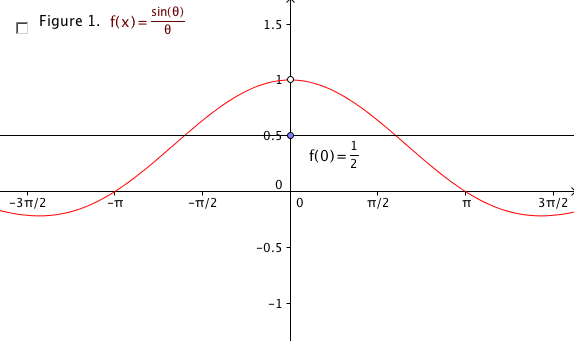
\includegraphics[scale=0.4]{singraph}}\\

Another interesting feature to note: although this function approaches a general limit of 1 as $\theta \to 0$ from both the left and the right, the actual value of $f(0) = \frac{1}{2}$.\\
\\
As x approaches infinity $f (\theta) \to 0$ (figure 2.)\\
%
{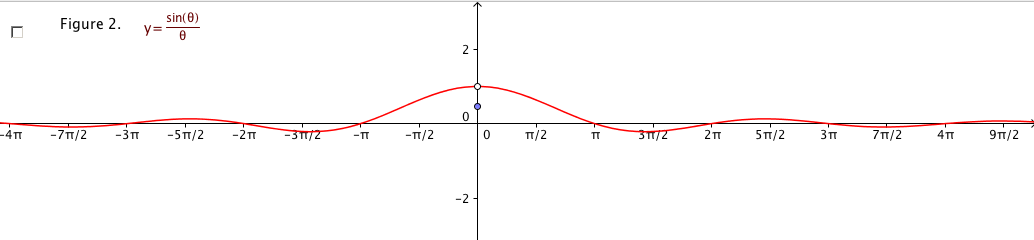
\includegraphics[scale=0.45]{longview}}\\


\vspace{8 mm}

{\bfseries 2. Examine the function below:}\\
\\
\fbox{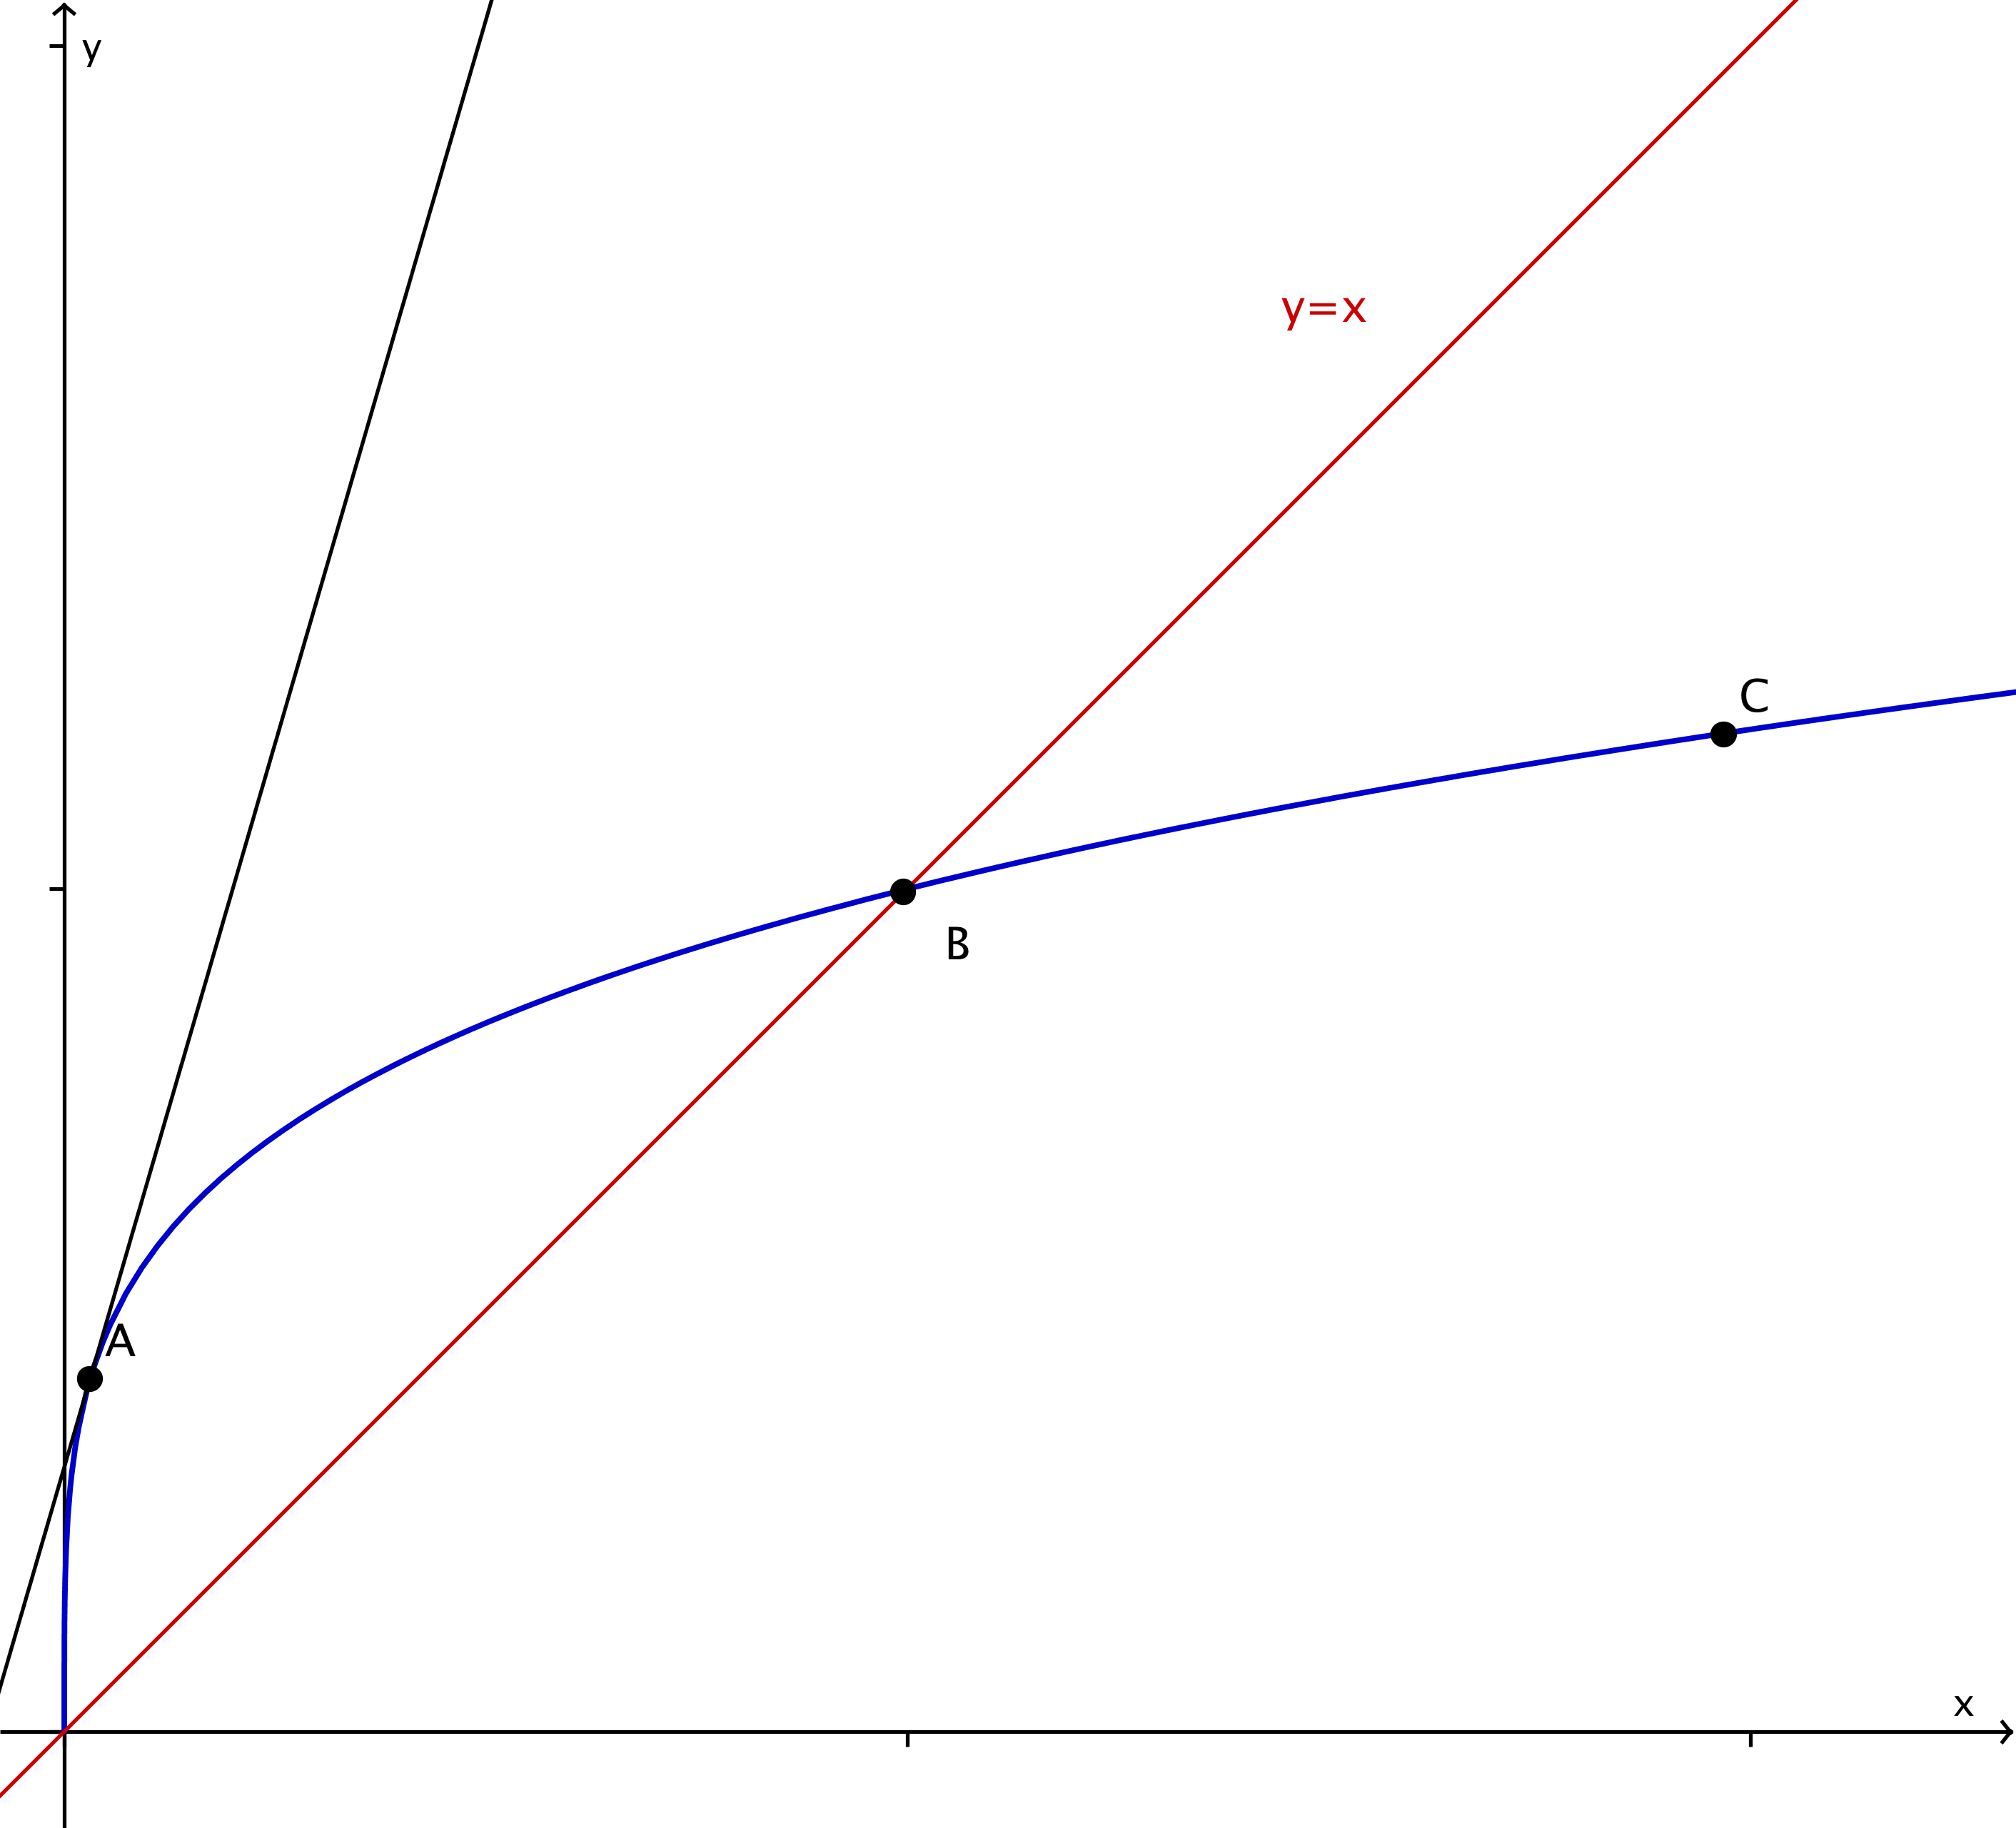
\includegraphics[scale=0.4]{loggy}}\\
%
\\Given only the information contained in the graph, is it possible to arrange the following quantities in increasing order? 
%
\begin{itemize}
%
	\item The slope of the tangent line to the graph at point A
	\item The slope of the tangent line to the graph at point B
	\item The slope of the tangent line to the graph at point C
	\item The slope of the line that contains points A and B
	\item The number 0
	\item The number 1
%	
\end{itemize}
The function appears to be of the form$f(x)= \sqrt{x}$ but no explicit formula is given nor are the axes enumerated. The coordinates of the points (A,B, and C) have also been withheld.  \\

Before we despair, let's take inventory of what we \emph have been given: The $x$ and $ y$ axes, and the line {\color{red}$y = x$} which is all the information we need to derive our slopes. \\

Recall, the slope of a line is calculated by the change in $y$ of a line over the change in $x$ also known as, $\frac{\text \bfseries RISE}{\text \bfseries RUN}$.
A line with the equation $y=x$ therefore has a slope of 1 as will any line parallel to it.\\ The x axis and lines parallel to it have a slope of zero. From this we can infer that lines which fall between the x axis and the line $y=x$ have slopes that are proper fractions (they rise fewer than one unit per unit of distance travelled.) Conversely, lines that fall between line $y=x$ and the $y$ axis are improper fractions that increase in slope the closer they parallel the $y$ axis (though lines {\emph exactly} parallel to the $y$ axis have an undefined slope. \\

Now lets arrange our items in increasing order. 0 is the smallest as we have no negative quantities, next we need to find the lines most closely parallel to the $x$ axis which will be slightly greater than 0 yet $< 1$.

\pagebreak

View figure 2.3.\\
\fbox { 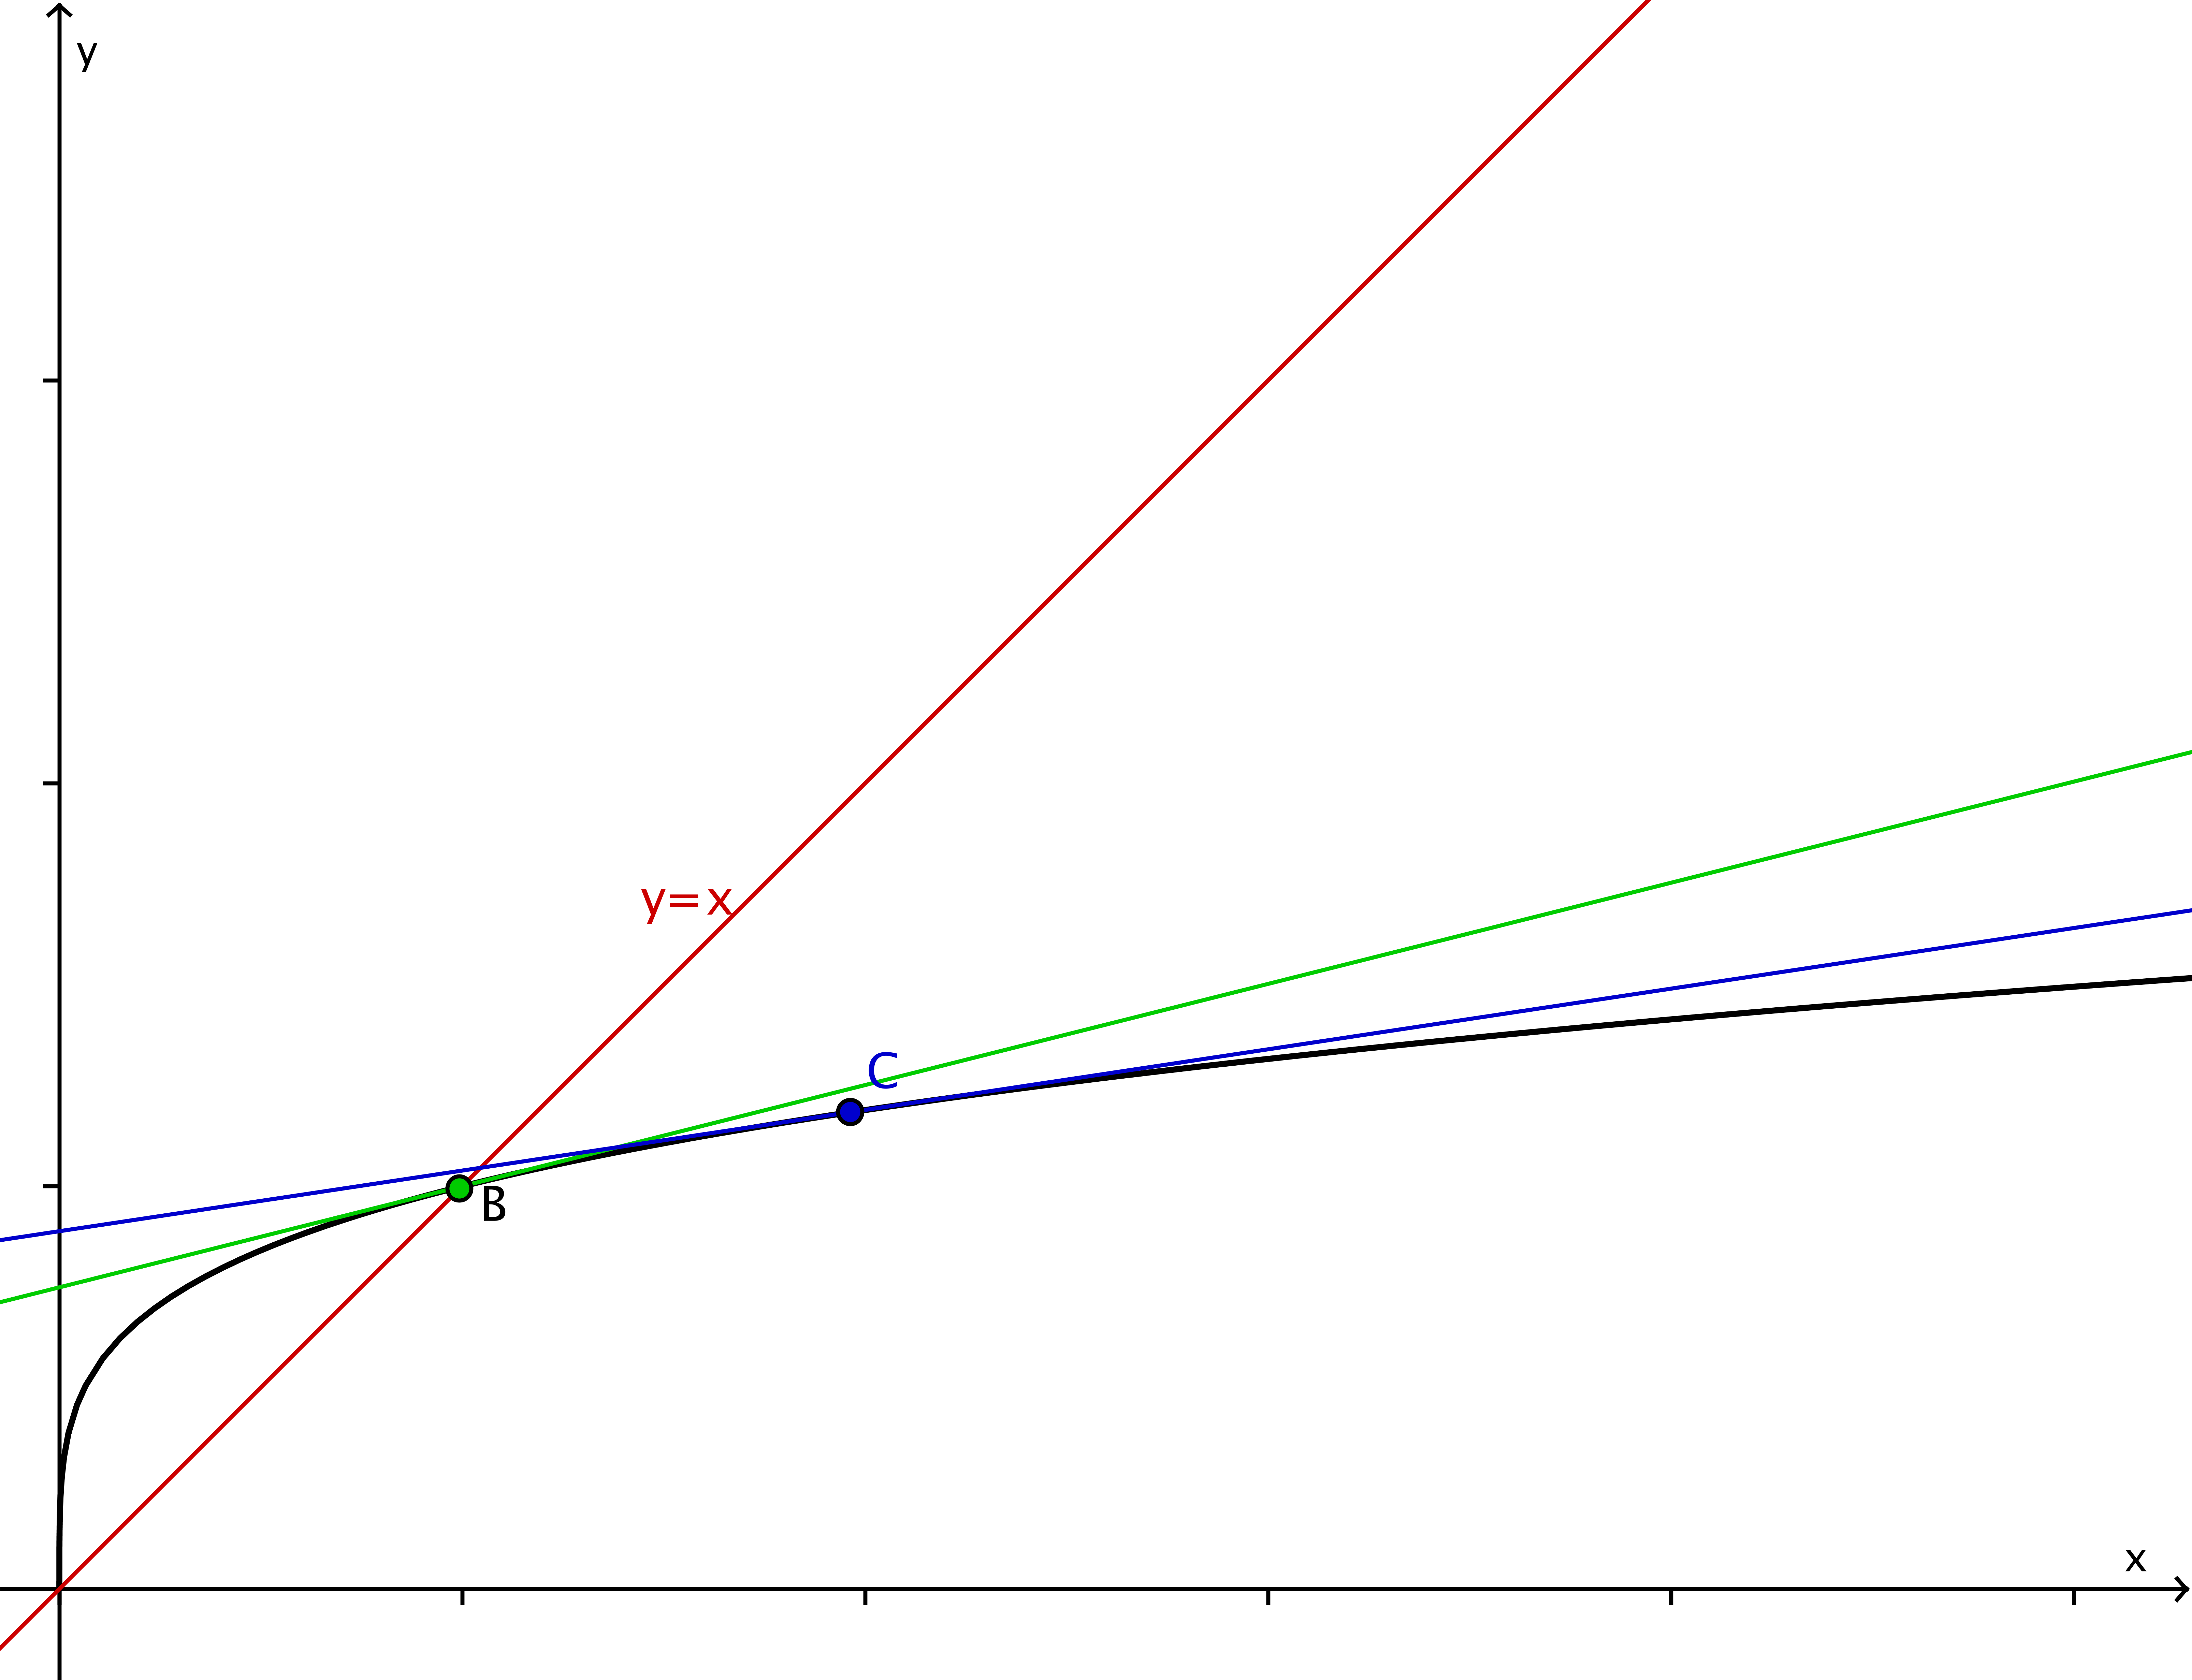
\includegraphics [scale= 0.19] {AB} } \\ 

Recall, a tangent line to a curve is a line that touches it at only one point and is the curves best straight line approximation \emph{at that point}. I have drawn color coded tangent lines at points { \color{green}{B}} and {\color{blue}{C}} on the graph 2.3.  Both lines lie between {\color{red} $y=x$} and the $x$ axis and thus have a slope $< 1$. The tangent line to point {\color{blue}{C}} most closely parallels the x axis and therefore is our second smallest quantity followed by the tangent line to { \color{green}{B}}. \\

We can assess our final quantities with figure 2.3\\
\fbox{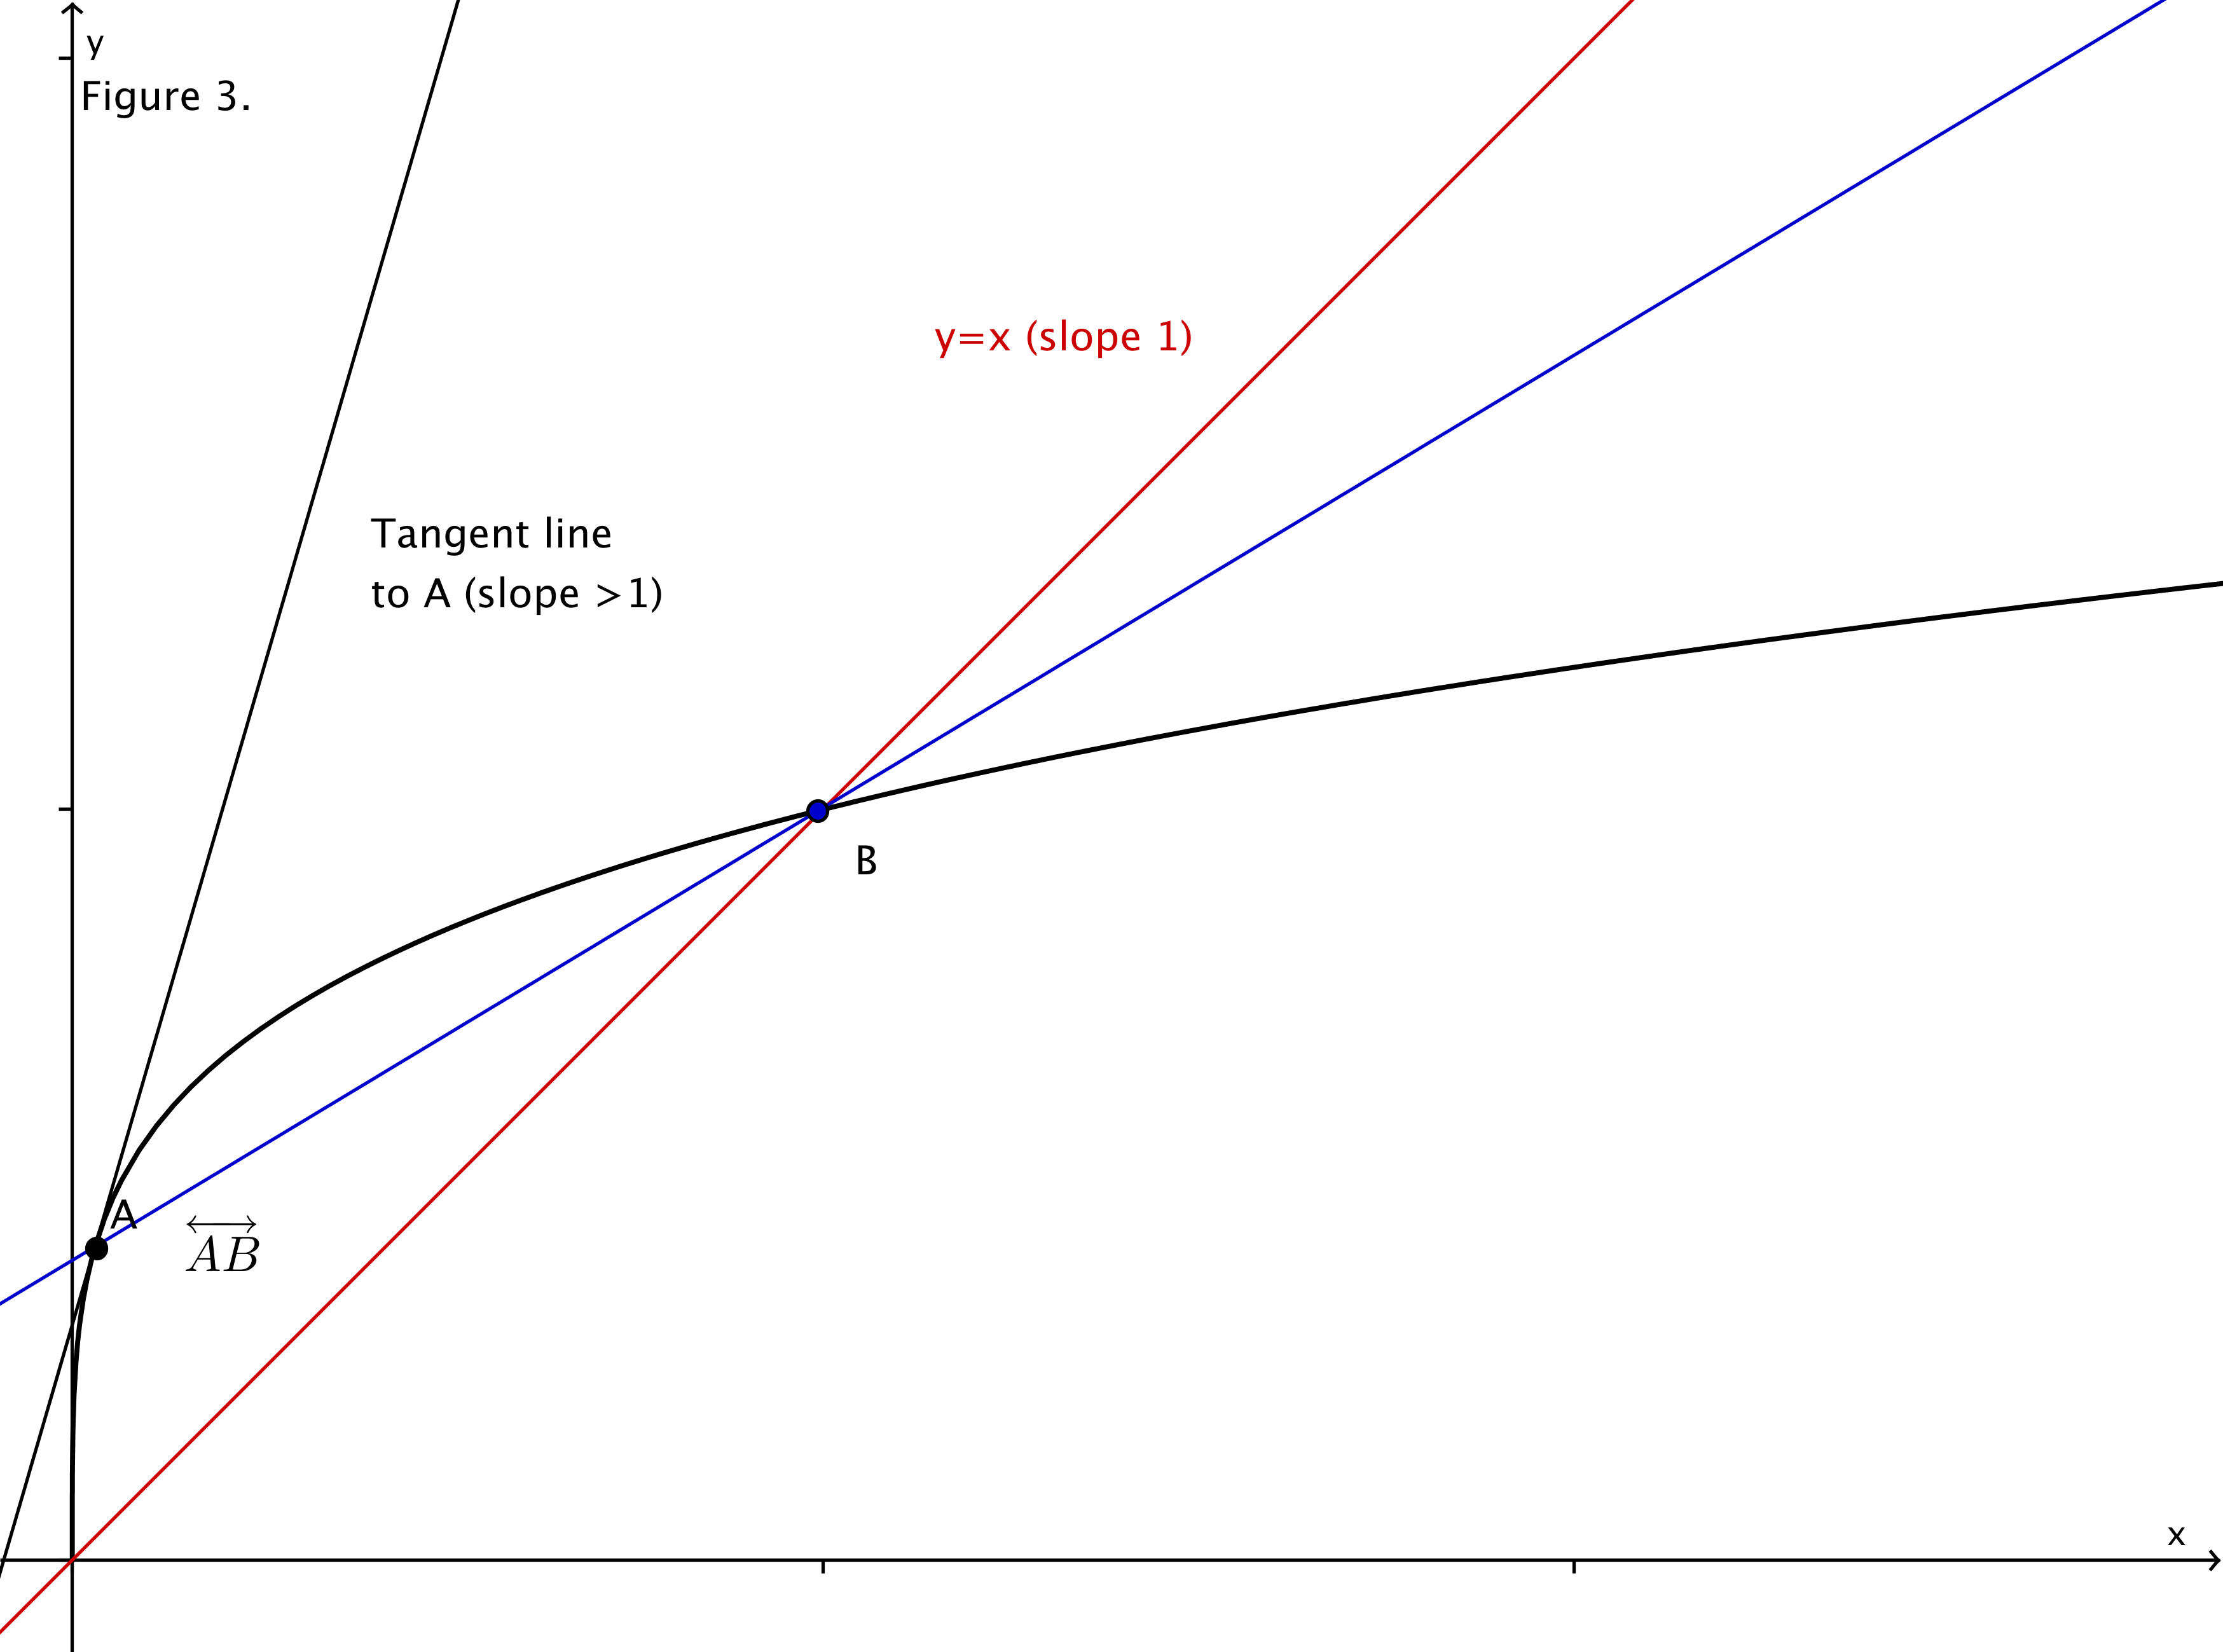
\includegraphics[scale= 0.35]{slopey}}\\ 
  
The tangent line to point A is the closest to the $y$ axis and our only quantity $ > 1$, as the line $\overleftrightarrow{AB}$ also falls between $y=x$ and the $x$ axis but is nearest to the line $y=x$. \\
{\bfseries We now can arrange our quantities in increasing order: 0, TanC, TanB, $\overleftrightarrow{AB}$, 1, and TanA.}
 
\end{enumerate}

{\bfseries 3. a. The Figure below is known as Pascal's Triangle.} It has many interesting and useful properties,\\ a few of which are: \\
\begin{itemize}
\item The edges are all the number 1. The diagonals beginning with the second row from the top are the counting numbers 1,2,3,4 . . .  \\
\item If you look at the digits of the pyramid, the horizontal rows are powers of 11( $11^0=1$,  $11^1= 11$, $11^2=121$,  $11^3=1331$, etc.) and the whole array is left/right symmetric. \\ 
\item The top row that is the single digit ``1'' is known as the ``zeroth'' row. The {\bfseries first} row begins the second line down from the top with the numbers 1, 1.
and the the second row contains 1,2,1 and so forth, It is {\bfseries very important} that we number correctly, as we shall see.
%
\end{itemize}
%
\mkPascal{8} \\

{\center {\bfseries b.} Watch what happens when we expand the following expressions:}
 
\begin{align*}
  (a + b)^0 &= 1\\
  (a + b)^1 &= a + b\\
  (a + b)^2 &= a^2 + 2ab + b^2\\
  (a + b)^3 &= a^3 + 3a^2b + 3ab^2 + b^3\\
  (a + b)^4 &= a^4 + 4a^3 b + 6a^2b^2 + 4ab^3 + b^4\\
  (a + b)^5 &= a^5 + 5a^4 b + 10a^3 b^2 + 10a^2 b^3 + 5ab^4+b^5
\end{align*} 

\vspace{3mm}
 
{\bfseries c.} The horizontal rows of Pascals Triangle correspond to the {\bfseries coefficients} of our binomial expansions. If a binomial is raised ti the $nth$ power you can look at the $nth$ row of the triangle to find the coefficients of its expansion. Example: $(a+b)^0 = 1$ as {\bfseries any} term raised to the zeroth power simply $=1$. For $(a+b)^2$ the coefficients are 1,2,1 the same as row 2 so  $(a+b)^2$ = ($(1) a^2+(2) ab+(1) b^2$.)
This means we can calculate the coefficients of any degree binomial expansion by simply referencing the corresponding row in Pascal's triangle, very cool! \\

\pagebreak   

\vspace{8 mm}

 {\bfseries d. The Quantity $(\frac{n}{k})$: The Number of Ways to Select {\emph k} Items From a Set of {\emph n} Objects.}\\
%
\vspace{4 mm}\\Say we have five Calculus gurus\textemdash Ann, Marisa, Amy, Kelly, and Steve whom we wish to arrange into pairs. In that case our quantity  $(\frac{n}{k})$ would be $(\frac{5}{2}).$
Let's see what the maximum number of unique (k) pairs that five (n) students can be put into.\\
\vspace{3 mm}

The formula to compute this is: 
\vspace{3 mm}
\[
 \binom{n}{k}=\frac{n!}{k!(n-k)!} \quad \text {Which in this case is:}  \quad \binom{5}{2}=\frac{5!}{2!(5-2)!}
\]
\vspace{3 mm}

The `` ! '' is called factorial and means the number before the ! is multiplied successively by all its predecessors back to the number one. Hence $3! = 3 \cdot 2 \cdot 1 = 6$.
\\ If we expand our formula we get:
\vspace{3 mm}
\[
 \binom{5}{2}=\frac{5!}{2! \cdot 3!} =\frac{5 \cdot 4 \cdot 3 \cdot 2 \cdot 1}{(2 \cdot 1)(3 \cdot 2 \cdot 1)}=\frac {120}{12} = 10
\]
\vspace{5 mm}
\begin{center} Our Calculus gurus can be paired up in 10 ways, which we can confirm:\\

\vspace{5 mm}
 \quad Steve, Amy. \quad Steve, Ann. \quad Steve, Marisa. \quad Steve, Kelly.\\ 
\vspace{2 mm}
\quad Amy, Ann.\quad Amy, Marisa. \quad Amy, Kelly.\\
\vspace{2 mm}
\quad  Ann, Marisa. \quad Ann, Kelly \\
\vspace{2 mm}
 \quad  Marisa, Kelly.\\ 
  
 \end{center}
 
 \pagebreak

  \vspace{3 mm}
 {\center{{\large \bfseries e. The Binomial Theorem.}}\\
 
   \vspace{2 mm}
 {\large A formula for expanding binomials of the form $(a+b)^n$}. \\ 
 
 \vspace{3 mm}
  
 \large  If n is a positive integer then:\\
\[
     (a+b)^n = \sum_{k=0}^n \binom{n}{k} a^{n-k} b^{k} \
\]

\vspace{2 mm} In the expression $\binom{n}{k}$ the upper index $n$, is the exponent of the binomial and the highest index of the series. The lower index $k$, indicates that the the series begins with $0$ and the $\sum$ means that you add all the terms indexed from 0 to $n$ together.
\vspace{2 mm}
For example: to expand  $(a + b)^5$  it will look like this:
\[
	\sum_{k=0}^5 \binom{5}{k} a^{5-k} \cdot b^{k}%\binom{5}{k}a^{5-k} \cdot b^k
\]

To calculate our variable expressions $5$ becomes the exponent of our first $a$ term and will count down from 5 to 0 each successive term$(5 - k)$, while the lower index $k$ becomes the exponent of $b$ and successively takes on ascending values of 0 through 5.\\

\vspace{2 mm}

(Terms with an exponent of 0 are ``invisible,'' as anything raised to the 0 power is equal to 1.)
\[
(a + b)^5 =\binom{5}{0} a^5(b^0)  +   \binom{4}{1}a^4b^1  +   \binom{3}{2}a^3b^2  +   \binom{2}{3}a^2b^3  +   \binom{1}{4}a^1 b^4  +   \binom{0}{5}(a^0) b^5
\]
Notice: The exponents of the $a$ and $b$ variables of each term of the series add up to 5; the original degree of our binomial.
Now that we have the exponents of the variables, how do we calculate the coefficient for each of the terms in the series?\\
\vspace{2 mm}
 You probably remember that we can use row five of Pascal's triangle (1, 5, 10, 10, 5, 1) and that is correct, but the answer is also right here in the theorem.\\
 we will use $\binom{n}{k}$ similar to how we derived all the unique pairings of five Calculus students in example d:
	\[
 \binom{n}{k}=\frac{n!}{k!(n-k)!}
	\]
\vspace{2 mm}As our index $k$ increases from 0 to 1 we obtain six different combinatorial possibilities: 
\[
\binom{5}{0}, \binom{5}{1}, \binom{5}{2}, \binom{5}{3}, \binom{5}{4}, \binom {5}{5}
\]

\vspace{2 mm}

$\binom{n}{0}= 1$, $\binom{n}{1}=n$, and $\binom{n}{n}=1$ so the first, second and last coefficients are easy: $\binom{5}{0}$ and $\binom{5}{5} $ both equal 1 and $\binom{5}{1}$ equals 5.
The next term $ \binom{5}{2}$ is identical to our Pairing of five students.\\
\[
 \binom{5}{2}=\frac{5!}{2! \cdot 3!} =\frac{5 \cdot 4 \cdot 3 \cdot 2 \cdot 1}{(2 \cdot 1)(3 \cdot 2 \cdot 1)}=\frac {120}{26} = 10
\]
\vspace{4 mm}\\ 

Continuing through the combinations we arrive at what we knew all along, the coefficients are identical to row five of Pascal's triangle. When we match them up with their corresponding variable expressions our complete expansion is:\\
	\[
	  	\mathbf {a^5  +  5a^4 b  +  10a^3 b^2  +  10a^2 b^3  +  5a b^4  +  b^5}
	\]
	
\vspace{4mm}	
	
{\bfseries f.} Now we will use all of our above knowledge to find an expression for the difference quotient of the function $f(x)=x^6$.\\

\vspace{3 mm}	

The difference quotient for $x^6$ is;

	\[
			\frac{(x + h)^6 +x^6}{h} \quad \text{ The binomial theorem tells us that:} 
	\]
\[
     (x+h)^6\quad=\quad \sum_{k=0}^6 \binom{6}{k} x^{6-k} h^{k} \
\]
\vspace{2 mm}

Which we may substitute into our difference quotient:\\

\[
          \frac{1}{h} \left\{ \left(\sum_{k=0}^6 \binom{6}{k} x^{6-k} h^{k}\right) - (x^6){}\right\}
\]
%
%
Expanding the binomial we achieve:

\vspace{2 mm}

 \[
	\frac{1}{h} \cdot \left\{(x^6 + 6x^5 h + 15x^4 h^2 + 20x^3 h^3 + 15x^2h^4+ 6x h^5 + h^6) - (x^6)\right\}	
\]

\vspace{3 mm}

The $ x^6$ terms cancel, we then factor an $h$ out of every term and cancel $\frac{1}{h}$.\\
			
\[
	\cancel{\frac{1}{h}} \cdot \cancel{h}( 6x^5  + 15x^4 h + 20x^3 h^2 + 15x^2h^3+ 6x h^4 + h^5)
\]

$=6x^5  + 15x^4 h + 20x^3 h^2 + 15x^2h^3+ 6x h^4 + h^5$\\

\vspace{7mm}

{\bfseries Our difference quotient is complete and is: $\mathbf {6x^5  + 15x^4 h + 20x^3 h^2 + 15x^2h^3+ 6x h^4 + h^5}$}\\

\vspace{8mm}

To find the derivative we can take the limit as $h\to0$:
	\[
		\lim_{h \to 0} (6x^5  + 15x^4 h + 20x^3 h^2 + 15x^2h^3+ 6x h^4 + h^5)
	\]
	\[
		\mathbf{= 6x^5}
		\]
				
 \end {document}
